
\chapter{Introduction\label{ch:intro}}

Our understanding of fundamental particles and interactions has progressed much from the early days.
These beginnings could be with Empdocles and his four roots fire, earth, air, and water, or with
Aristotle relating these four roots to two of the four sensible quantities hot, dry, wet, and
cold~\cite{0415078547} as in Figure~\ref{fig:aristotle}
(not to omit classical elements from other philosophies and worldviews), or more recently with
John Dalton's atoms~\cite{dalton}. Or perhaps particle physics began with
the discovery of the electron by J.J. Thomson in 1897~\cite{thomson:electron},
which to this day has not been observed
to have internal structure or decay, with upper (lower) bounds on the radius (lifetime) of
10$^{-22}$~m (10$^{26}$~years)~\cite{1988PhST...22..102D,2002PhLB..525...29B}.

\begin{figure}[ht]
 \begin{center}
    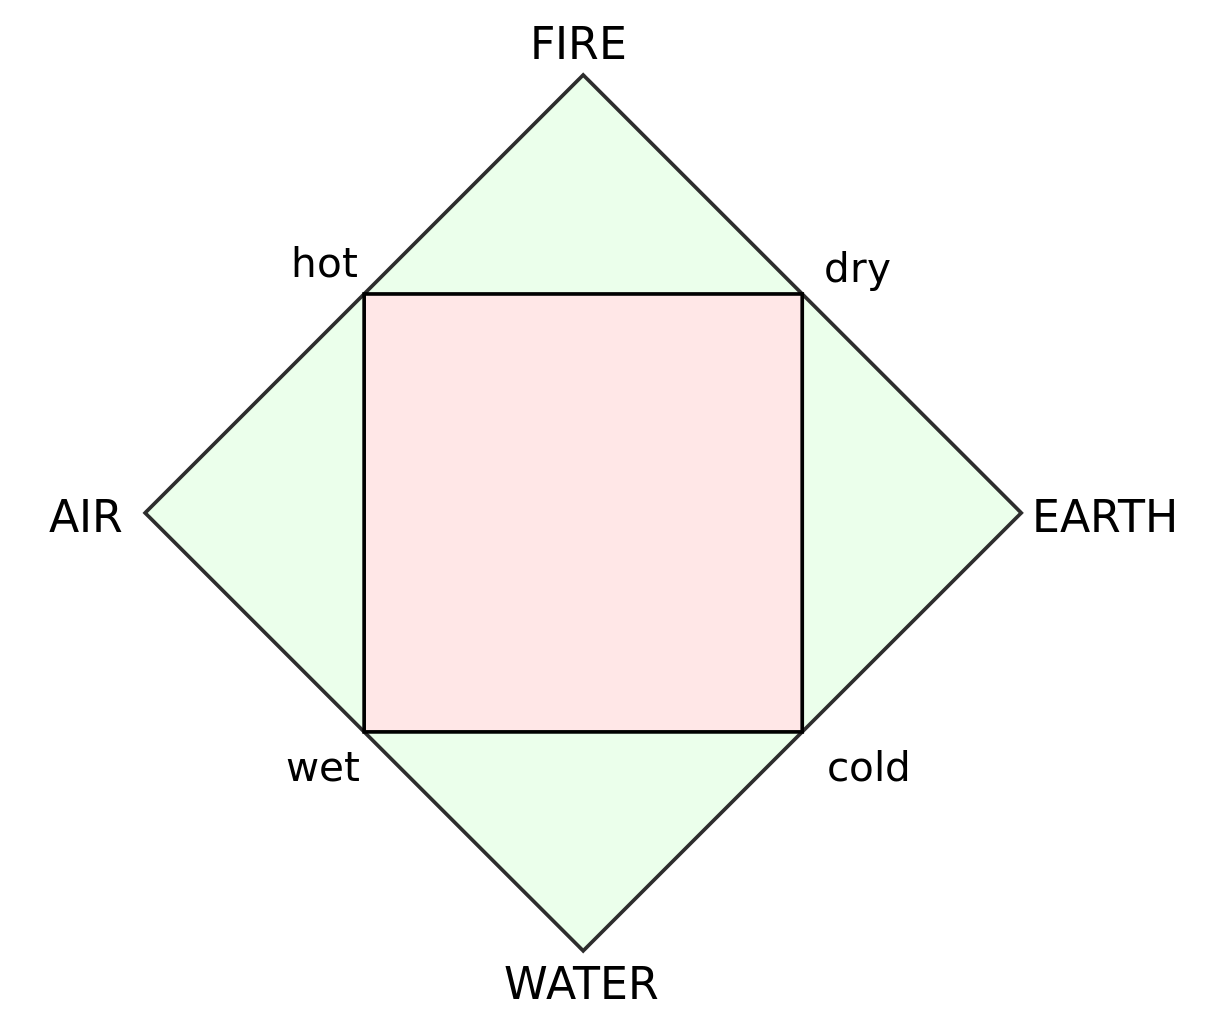
\includegraphics[width=0.90\textwidth]{figures/intro/Four_elements_representation.png}
      \end{center}
\caption{The four roots how they relate to the sensible quantities.}
\label{fig:aristotle}
\end{figure}

Today we have the Standard Model, the theoretical framework that best describes the
experimentally oberserved phenomena of the fundamental particles and their interactions. The theory
is not perfect, and it remains an overarching theme of particle physics to unify physical processes
at all energy scales under one single framework, if such a thing can be done at all.
The SM, its successes, and its shortcomings are described in
Sections~\ref{sec:SM}, \ref{sec:SMsuccess}, and \ref{sec:SMshortcomings}.

Recently in 2012, the last piece to the SM was put into place with the discovery of the Higgs boson.
This discovery, described in Section~\ref{sec:discovery}, is the foundation for the work based on
this thesis, the goal of which is to describe the first search for diHiggs production, a process
in which two Higgs bosons are produced. The motivations for what the search for this process means
in the context of SM physics and ``new'' physics is given in Section~\ref{sec:diHiggs}.

Finally, for those readers who have by chance come across this thesis and do not
have any physics training, Appendix~\ref{ch:mom} may be especially appealing.

\section{The Standard Model\label{sec:SM}}

The Standard Model (SM) of particle physics is a relativistic quantum field theory
that describes how the known fundamental particles interact through the electromagnetic, weak,
and strong forces.
The theory was developed through the unification of the electromagnetic and weak forces by Glashow
in 1961~\cite{1961.Glashow.Partial-symmetries} and through the incorporation of this electroweak
theory with the Higgs mechanism by Weinberg and Salam in 1967~\cite{PhysRevLett.19.1264,Salam:1968rm}.
This theory explained the experimental observations of the day, and later experiments provided
additional evidence as well as a mean for measuring the free parameters of the theory. Some of
this evidence is provided in Figure~\ref{fig:discoveries} in the form of the discoveries of
the fundamental particles.

\begin{figure}[ht]
 \begin{center}
    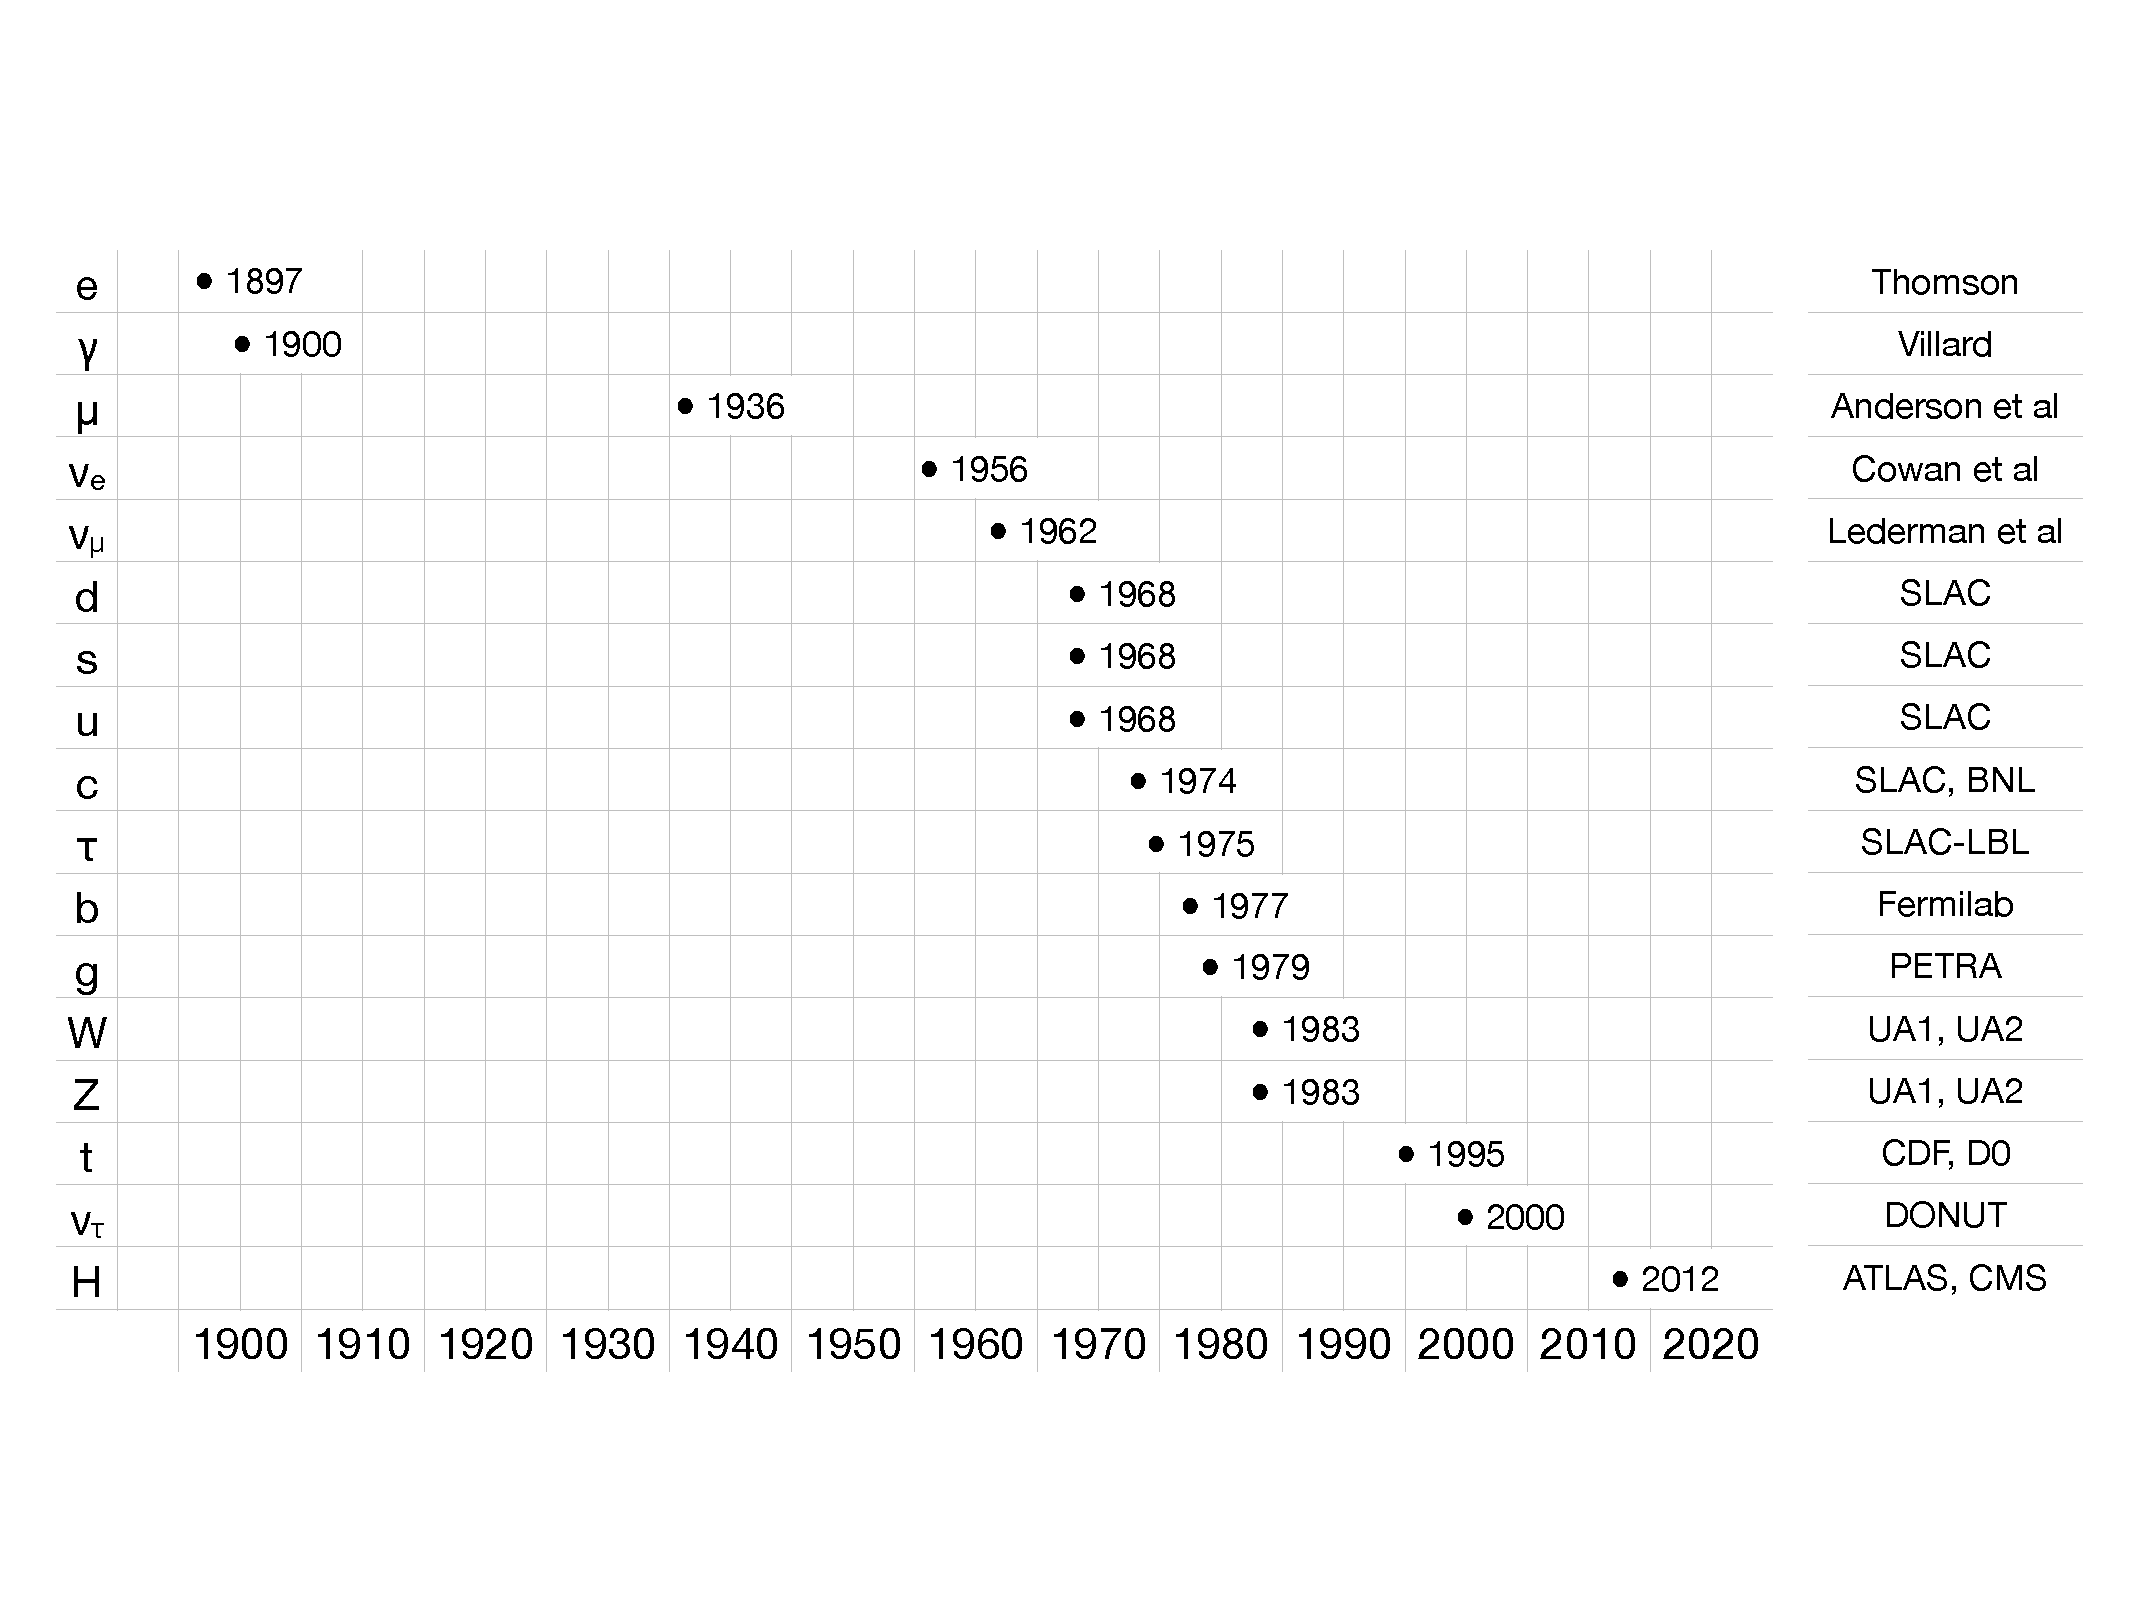
\includegraphics[width=0.90\textwidth]{figures/intro/discoveries.pdf}
      \end{center}
\caption{The discoveries of fundamental particles versus time~\cite{Tuna:thesis}.}
\label{fig:discoveries}
\end{figure}

In this theory, particles are treated as excitations of fields having half-integer spin or
integer spin, and the forces are treated as interactions among excitations of these fields.
The spin-$\frac{1}{2}$ particles, or fermions, can be divided into groups based on the ways
in which they interact. The leptons, or those particles which only experience the electroweak force,
are the electron $e$, muon $\mu$, tau $\tau$, electron neutrino $\nu_e$, muon neutrino $\nu_\mu$, and
tau neutrino $\nu_\tau$. The quarks, or those particles which experience both electoweak and strong
forces, are the up $u$, down $d$, strange $s$, charm $c$, bottom $b$, and top $t$. The integer-spin
particles, or bosons, are the spin-1 photon $\gamma$, $W$, $Z$, and gluon $g$ and the spin-0 Higgs $H$.
The particle content of the SM is summarized in Figure~\ref{fig:SMtable}.

\begin{figure}[ht]
 \begin{center}
    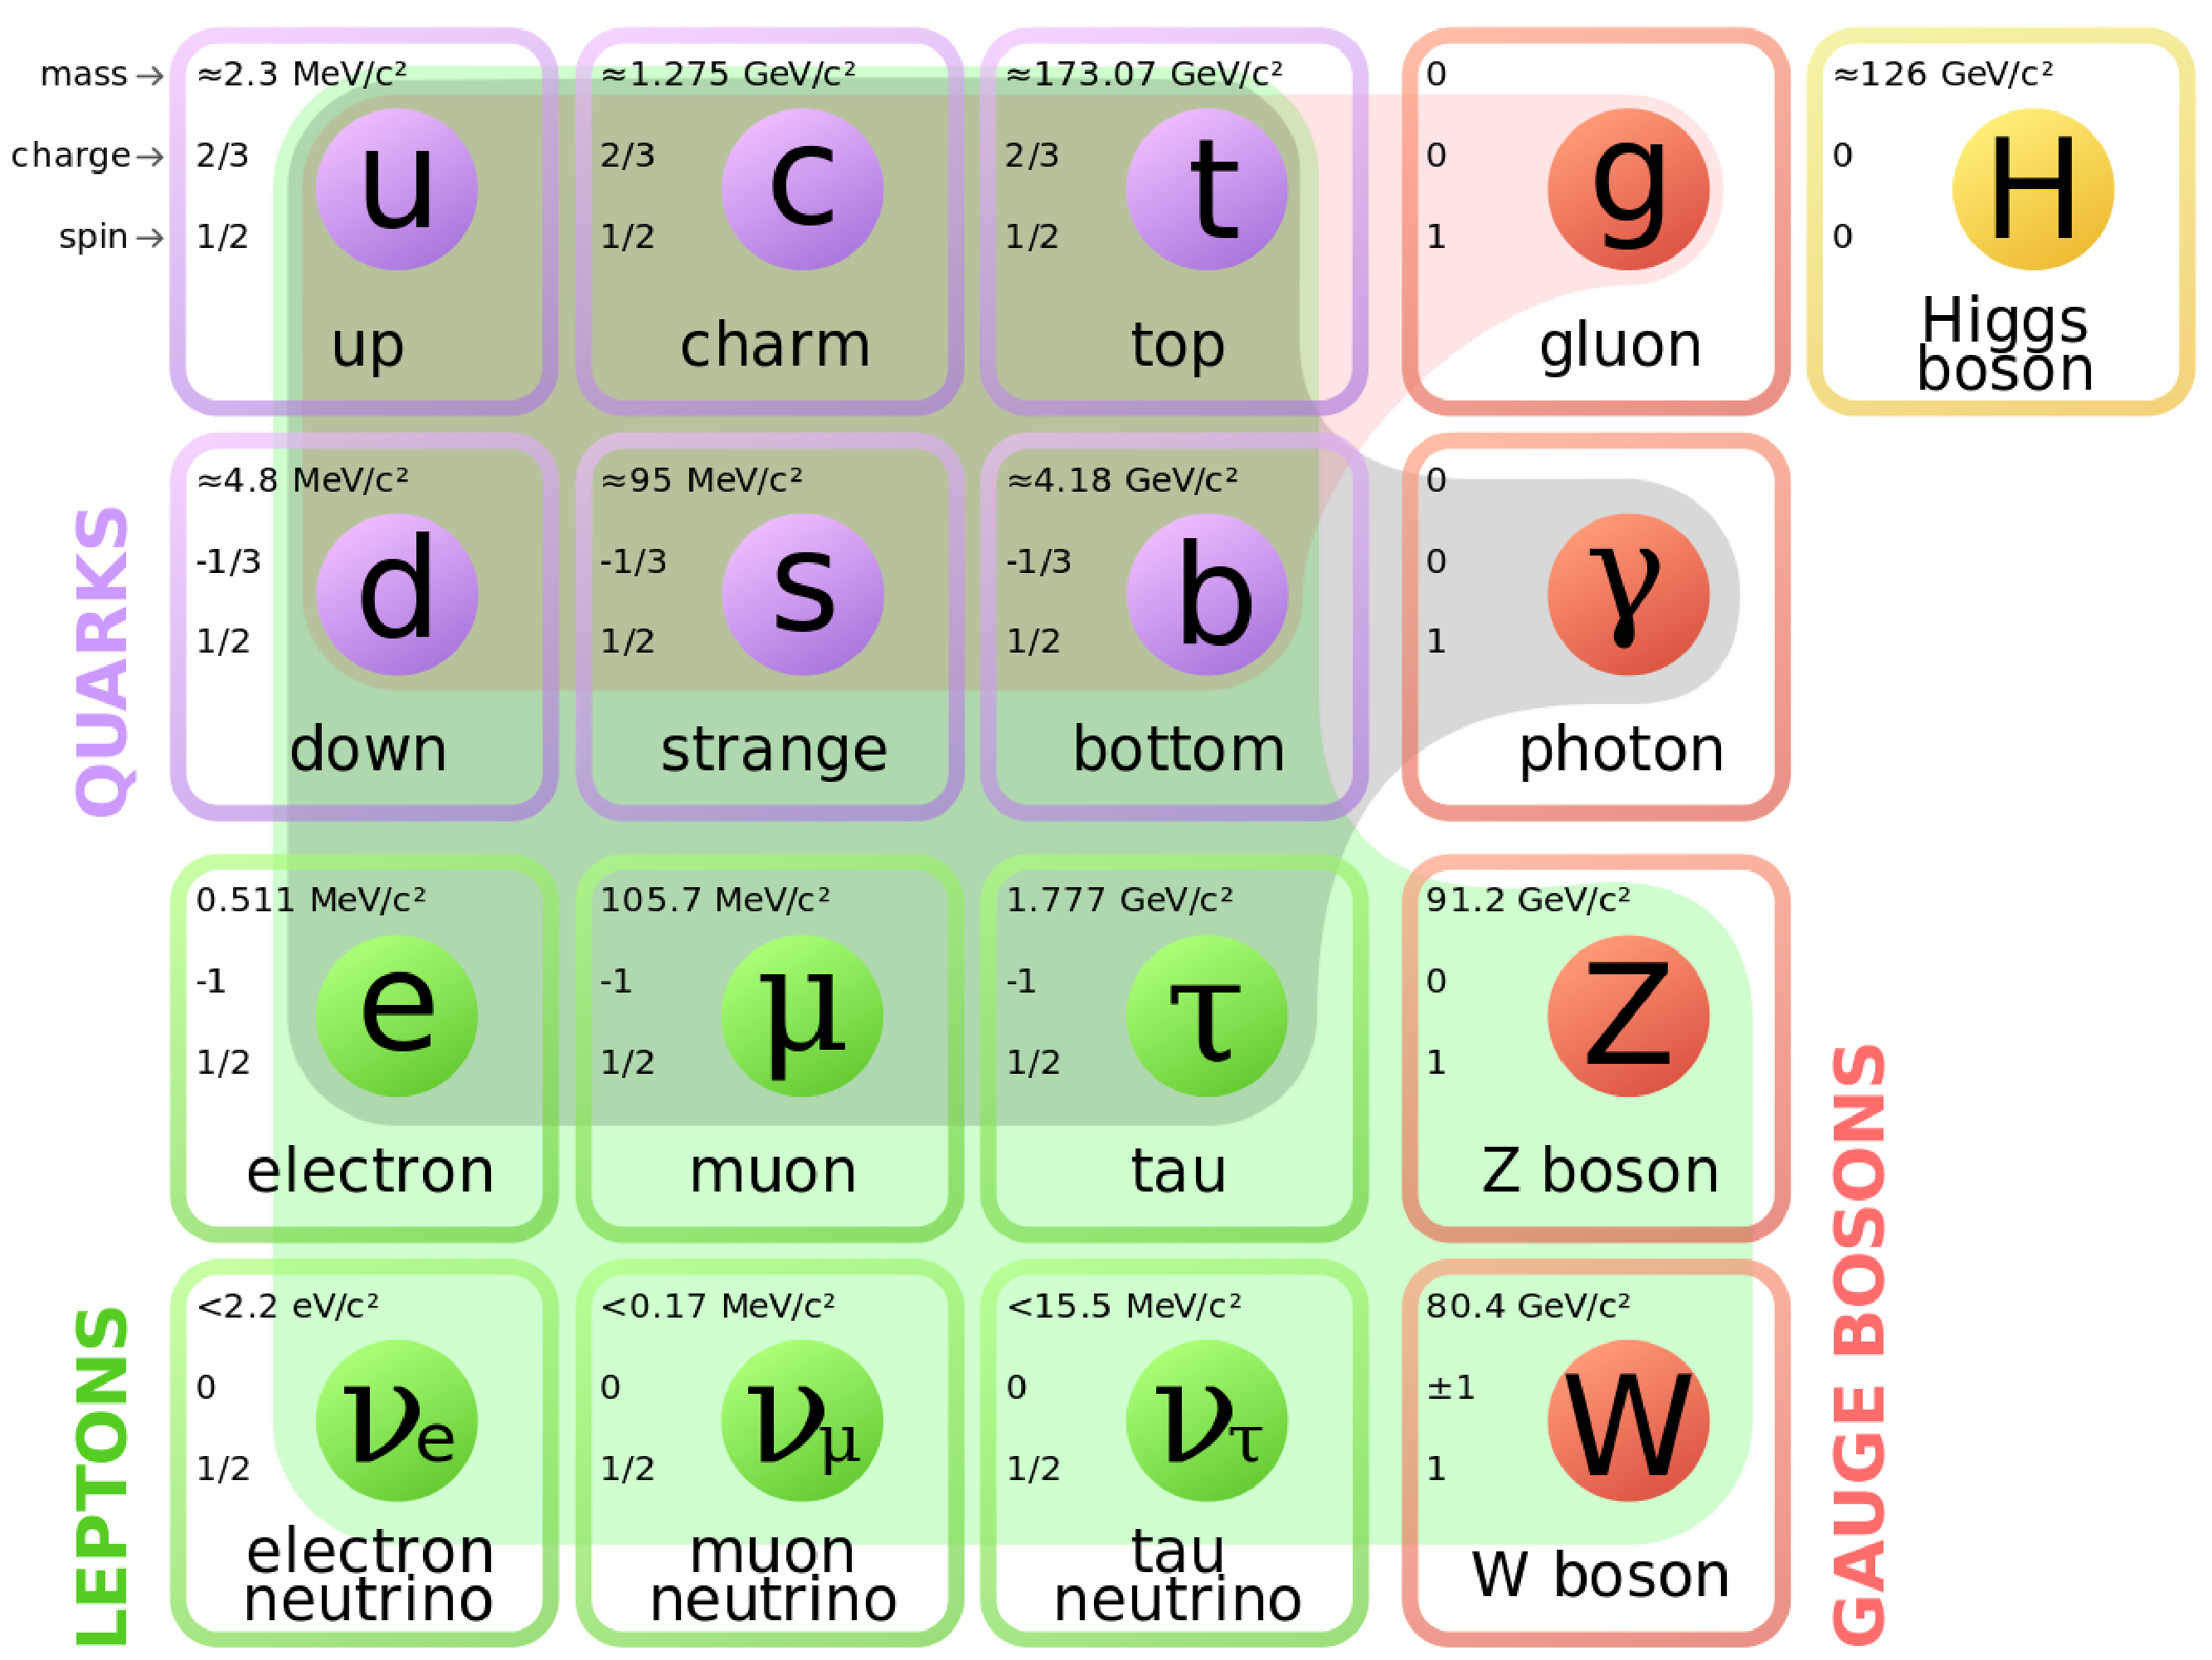
\includegraphics[width=0.90\textwidth]{figures/intro/Standard_Model_of_Elementary_Particles_modified_version.pdf}
      \end{center}
\caption{A diagram of the particle content of the SM~\cite{SMdiagram}.
The mass, electric charge, and spin is given for each, and the background color indicates how each
fermion interacts with the bosons.}
\label{fig:SMtable}
\end{figure}

The dynamics of the SM are described through its Lagrangian, which is invariant under
gauge transformations of the group ${\rm SU(3)}_C \times {\rm SU(2)}_L \times {\rm U(1)}_Y$.
The strong force is associated with transformations under ${\rm SU(3)}_C$, which give rise to
the conserved color charge $C$, denoted red, green, or blue, and eight gauge fields.
The group acts on 18 spinor fields corresponding to the quarks (six quark flavors in three colors)
and the eight gauge fields corresponding to the gluons.
The electroweak force is associated with transformations under ${\rm SU(2)}_L \times {\rm U(1)}_Y$,
the first part of which give rise to the conserved left-handed chirality $L$ and three gauge fields,
and the second part of which gives rise to the conserved weak hypercharge $Y$ one gauge field.
This group acts on left-handed doublets and right-handed singlets of the quarks, leptons, and
these four gauge fields. The quarks contribute nine doublets and 18 singlets, and the leptons contribute
three doublets and three singlets (as right-handed neutrinos do not exist).

The symmetry group of the SM does not allow for gauge-invariant mass terms. Instead,
the generation of particle masses is accomplished through the partial breaking of the
symmetry group by the addition of the Higgs field and potential, after which gauge-invariant
Yukawa interactions between fermions and the Higgs field naturally give fermion masses.
The Higgs field $\phi$ is a doublet of ${\rm SU(2)}_L$, and its potential takes the form

\begin{equation}
V(\phi^\dagger\phi) = -\mu\phi^\dagger\phi + \lambda(\phi^\dagger\phi)^2 ,
\end{equation}

where $\mu,\lambda > 0$.

\section{Higgs Discovery\label{sec:discovery}}
reference by sec:CMS

\section{Successes of the SM\label{sec:SMsuccess}}

\section{Shortcomings of the SM\label{sec:SMshortcomings}}
reference by sec:CMS


\section{diHiggs as a probe of SM and New Physics\label{sec:diHiggs}}


